\begin{enumerate}
\item Consider the relation $\relA$ defined by 
$ \relA = \{ (x,y) \suchthat \; x \, \mbox{has the same astrological sign as} \, y \}$.  Show that $\relA$ is an equivalence relation.  What equivalence class
under $\relA$ do you belong to?
\item Define a relation $\square$ on the integers by $x \square y \; \iff x^2 = y^2$.  Show that $\square$ is an equivalence relation.  List the equivalence
classes $x/\square$ for $0 \leq x \leq 5$.
\item Define a relation $\relA$ on the set of all words by

\[ w_1 \relA w_2 \quad \iff \quad w_1 \mbox{ is an anagram of } w_2. \]

\noindent Show that $\relA$ is an equivalence relation.  (Words are anagrams
if the letters of one can be re-arranged to form the other.  For example, `ART' and `RAT' are anagrams.)
\item The two diagrams below both show a famous graph known as the 
\index{Petersen graph}Petersen graph.  The picture on the 
left is the usual representation which emphasizes its five-fold symmetry.  The picture on the right
highlights the fact that the Petersen graph also has a three-fold symmetry.  Label the right-hand diagram
using the same letters (A through J) in order to show that these two representations are truly isomorphic.

\vspace{.2in}

\rule{0pt}{0pt} \hspace{-.75in} \begin{picture}(0,0)%
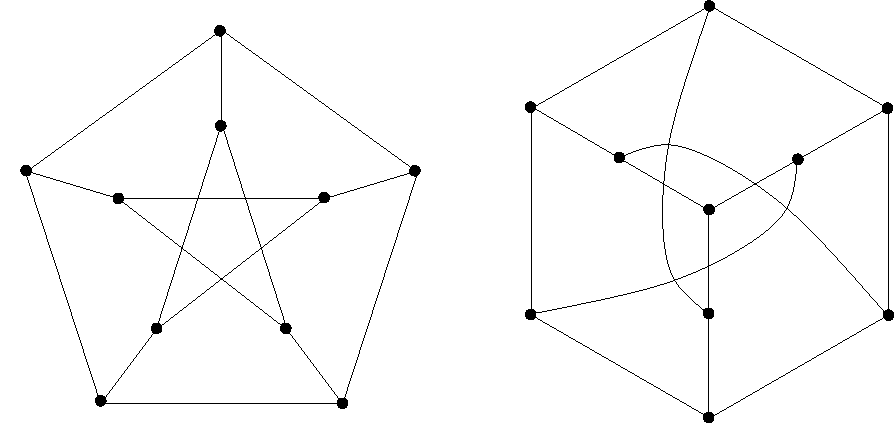
\includegraphics{./petersen_iso.pdf}%
\end{picture}%
\setlength{\unitlength}{3947sp}%
%
\begingroup\makeatletter\ifx\SetFigFont\undefined%
\gdef\SetFigFont#1#2#3#4#5{%
  \reset@font\fontsize{#1}{#2pt}%
  \fontfamily{#3}\fontseries{#4}\fontshape{#5}%
  \selectfont}%
\fi\endgroup%
\begin{picture}(7159,3450)(1453,-8445)
\put(3280,-5177){\makebox(0,0)[lb]{\smash{{\SetFigFont{12}{14.4}{\familydefault}{\mddefault}{\updefault}{\color[rgb]{0,0,0}A}%
}}}}
\put(4846,-6295){\makebox(0,0)[lb]{\smash{{\SetFigFont{12}{14.4}{\familydefault}{\mddefault}{\updefault}{\color[rgb]{0,0,0}B}%
}}}}
\put(4231,-8422){\makebox(0,0)[lb]{\smash{{\SetFigFont{12}{14.4}{\familydefault}{\mddefault}{\updefault}{\color[rgb]{0,0,0}C}%
}}}}
\put(2126,-8430){\makebox(0,0)[lb]{\smash{{\SetFigFont{12}{14.4}{\familydefault}{\mddefault}{\updefault}{\color[rgb]{0,0,0}D}%
}}}}
\put(1468,-6280){\makebox(0,0)[lb]{\smash{{\SetFigFont{12}{14.4}{\familydefault}{\mddefault}{\updefault}{\color[rgb]{0,0,0}E}%
}}}}
\put(3316,-5978){\makebox(0,0)[lb]{\smash{{\SetFigFont{12}{14.4}{\familydefault}{\mddefault}{\updefault}{\color[rgb]{0,0,0}F}%
}}}}
\put(4116,-6756){\makebox(0,0)[lb]{\smash{{\SetFigFont{12}{14.4}{\familydefault}{\mddefault}{\updefault}{\color[rgb]{0,0,0}G}%
}}}}
\put(3839,-7661){\makebox(0,0)[lb]{\smash{{\SetFigFont{12}{14.4}{\familydefault}{\mddefault}{\updefault}{\color[rgb]{0,0,0}H}%
}}}}
\put(2244,-6796){\makebox(0,0)[lb]{\smash{{\SetFigFont{12}{14.4}{\familydefault}{\mddefault}{\updefault}{\color[rgb]{0,0,0}J}%
}}}}
\put(2519,-7663){\makebox(0,0)[lb]{\smash{{\SetFigFont{12}{14.4}{\familydefault}{\mddefault}{\updefault}{\color[rgb]{0,0,0}I}%
}}}}
\end{picture}%


\vspace{.2in}

\clearpage

\item We will use the symbol $\Integers^{\ast}$ to refer to the set of
all integers \emph{except} $0$.  
Define a relation $\relQ$ on the set of all pairs in $\Integers \times \Integers^{\ast}$ (pairs of integers where the second coordinate is non-zero) by
$(a,b) \relQ (c,d) \; \iff \; ad=bc$.  Show that $\relQ$ is an 
equivalence relation.

\item The relation $\relQ$ defined in the previous problem partitions
the set of all pairs of integers into an interesting set of equivalence
classes.  Explain why 

\[ \Rationals \quad = \quad (\Integers \times \Integers^{\ast}) / \relQ. \]

\noindent Ultimately, this is the ``right'' definition of the set 
of rational numbers!

\item Reflect back on the proof in problem 5.  Note that we were fairly
careful in assuring that the second coordinate in the ordered pairs is
non-zero. (This was the whole reason for introducing the 
$\Integers^{\ast}$ notation.)  At what point in the argument did you
use this hypothesis?

\end{enumerate} 

%% Emacs customization
%% 
%% Local Variables: ***
%% TeX-master: "GIAM-hw.tex" ***
%% comment-column:0 ***
%% comment-start: "%% "  ***
%% comment-end:"***" ***
%% End: ***
